\section{$PSF$ approximation for parallel and distributed deconvolution} \label{gradients}
Because of the Major cycle, we already use an approximate $PSF$.

For a distributed deconvolution, we would like to deconvolve the image with as little communication as possible. This largely depends on the size of the $PSF$ when compared to the overall image. If the $PSF$ is for example $\frac{1}{16}$ of the total image size, we have patches of the image which are completely independent of each other. Sadly, this is not true for radio interferometers. The $PSF$ is generally the same size as the image. We cannot deconvolve any part of the image independently of each other.

However, we have two effects of modern radio interferometers, that produce an "approximately" smaller $PSF$: First, we have an increasing number of visibilities. They create a $PSF$ that increasingly resembles a Gaussian function in the center, and the rest approaches zero. And secondly, we reconstruct images with a wide field-of-view. Although the $PSF$ is not zero the further away we move from the center, its values approach zero.

\begin{figure}[h]
	\centering
	\begin{subfigure}[b]{0.3\linewidth}
		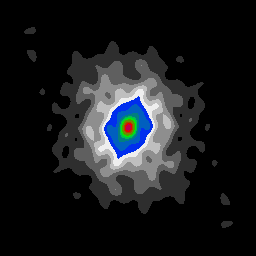
\includegraphics[width=\linewidth]{./chapters/03.distribution/simulated/psf.png}
	\end{subfigure}
	\begin{subfigure}[b]{0.3\linewidth}
		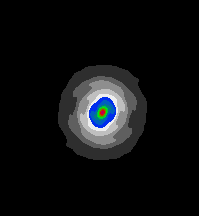
\includegraphics[width=\linewidth]{./chapters/06.gradient/psf_cut.png}
	\end{subfigure}
	
	\caption{$PSF$ arising from an increasing number of visibilities.}
\end{figure} 

In short, with an ever increasing number of visibilities and field-of-view, the influence of far-away image sections become negligible. We can approximate the deconvolution with a fraction of the true $PSF$. To our knowledge, we are the first to propose such approximation methods. In this Section, we present our approximation methods. In Section \ref{results:gradients}, we empirically demonstrate the validity of our approximations on a real-world MeerKAT observation. In Section \ref{pcdm}, we show more sophisticated coordinate descent methods that can exploit the smaller $PSF$. 

\subsection{Intuition for approximating the $PSF$}
Our basic coordinate descent algorithm chooses a pixel to minimize, calculates its gradient and descends in that direction. The gradient calculation reduces itself to a correlation of the residuals with the $PSF$ at the pixel location. In other words, we need the $PSF$ to calculate a gradient. If we only use parts of the $PSF$ for the calculation, we essentially approximate the gradient for the pixel. Because the $PSF$ only has significant non-zero values in the center, we should be able to ignore most of the values and still have an adequate gradient approximation.

%Introducing sparsity

Furthermore, our basic coordinate descent algorithm reconstructs inside the Major/Minor cycle framework. The framework is designed to handle only an approximate $PSF$ in the deconvolution (Remember: the $w$-term changes the $PSF$ depending on the position in the image). The framework may be able to deal with further $PSF$ approximations, namely with a $PSF$ that is reduced in size, which makes the distributed deconvolution simpler.

The approximation methods essentially work by "cutting off" the less significant $PSF$ values and only use a rectangle around the center. If we cut off the $PSF$ by a factor of $\frac{1}{4}$ (If the $PSF$ is $1024^2$ pixels in size, we only use a rectangle of $256^2$ of the center), we get pixels in the reconstructions that are not influenced by each other. Starting from a cut-off factor of $\frac{1}{16}$, we can split the image into eight patches, four of which are independent of each other. This would allow us to run up to four basic coordinate descent algorithms in parallel, simplifying the distribution.

Indeed, it is possible to approximate the $PSF$ with only a fraction of its true size, as we will demonstrate empirically in Section \ref{results:gradients}. But an approximation of the $PSF$ may lead to other problems in the reconstruction:
\begin{itemize}
	\item Needs additional Major cycles to converge.
	\item Slow down convergence speed of coordinate descent.
	\item Not guaranteed to converge to the same image.
\end{itemize}

The Major cycle corrects the errors the approximate $PSF$ introduces. The more inaccurate the $PSF$ is, the more Major cycles we may need to converge. As we already discussed, a Major cycle is an expensive operation. Our $PSF$ approximation should lead to as few (if any) additional Major cycles.

For the basic coordinate descent algorithm, an approximate $PSF$ may slow down the convergence speed. In each iteration, the basic algorithm finds the optimal value for the current pixel. With an approximate $PSF$, we may need several iterations on the same pixel (over several major cycles) until we arrive at the same value. In short, an approximate $PSF$ can slow down the convergence speed of coordinate descent.

Depending on how we approximate the $PSF$, we may not have any guarantee that we arrive at the same result. We developed two approximation methods: Method 1 uses an approximation in the gradient update step of coordinate descent. Method 2 solves an approximate deconvolution problem with only a fraction of the $PSF$. Only method 1 is guaranteed to converge to the same solution (with enough major cycles), but is slower to converge than method 2. Depending on the method we use, we can remedy some of the problems that approximating the $PSF$ introduces. But there seems to be a trade-off to be made. We have not found a method that works best in every aspect.

\subsection{Method 1: Approximate gradient update}
\begin{figure}[h]
	\centering
	\begin{subfigure}[b]{0.245\linewidth}
		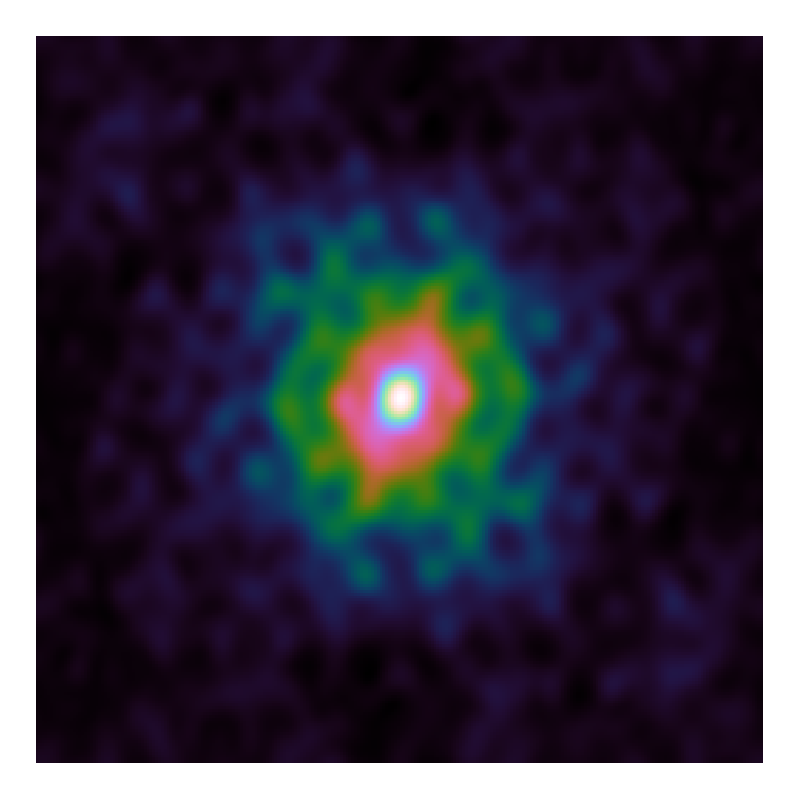
\includegraphics[width=\linewidth, clip, trim= 0.25in 0.25in 0.25in 0.25in]{./chapters/03.cd/simulated/psf.png}
		\caption{$PSF$}
	\end{subfigure}
	\begin{subfigure}[b]{0.245\linewidth}
		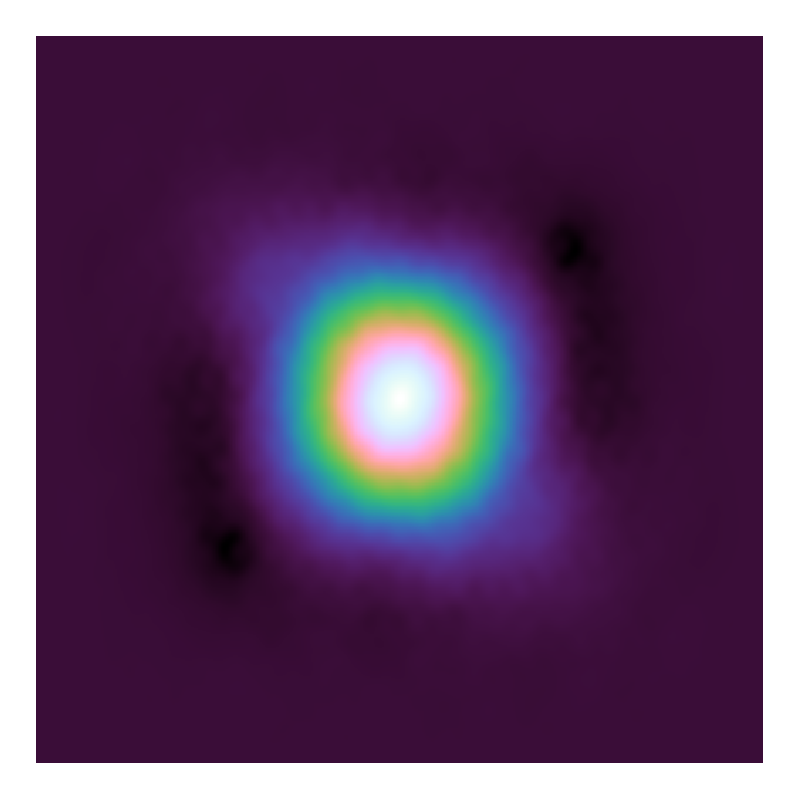
\includegraphics[width=\linewidth, clip, trim= 0.25in 0.25in 0.25in 0.25in]{./chapters/03.cd/simulated/psfSquared.png}
		\caption{Gradient update}
	\end{subfigure}
	\begin{subfigure}[b]{0.245\linewidth}
		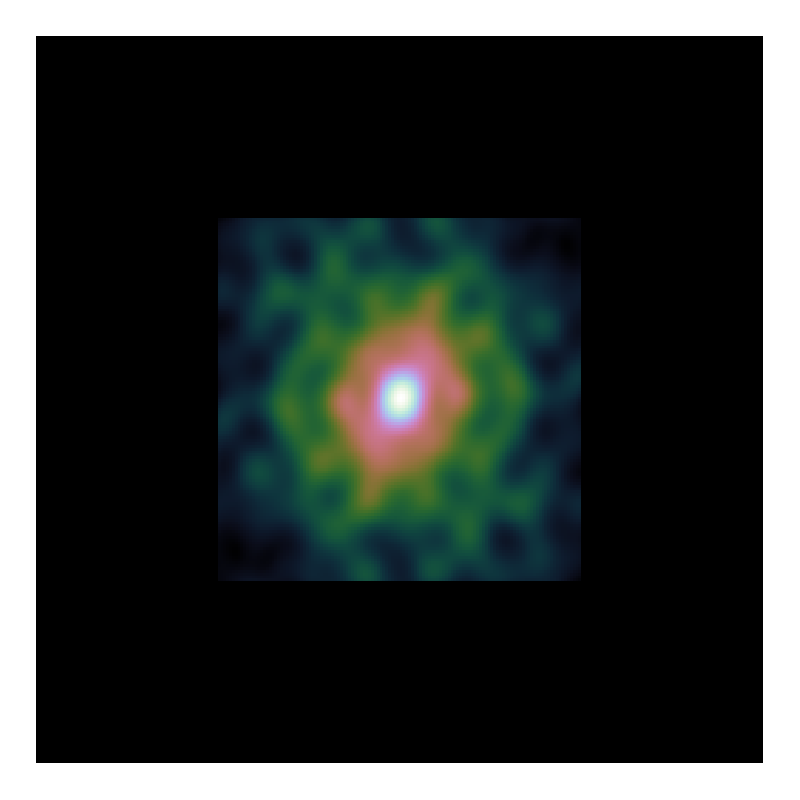
\includegraphics[width=\linewidth, clip, trim= 0.25in 0.25in 0.25in 0.25in]{./chapters/03.cd/simulated/psfCut.png}
		\caption{$cut(PSF)$}
	\end{subfigure}
	\begin{subfigure}[b]{0.245\linewidth}
		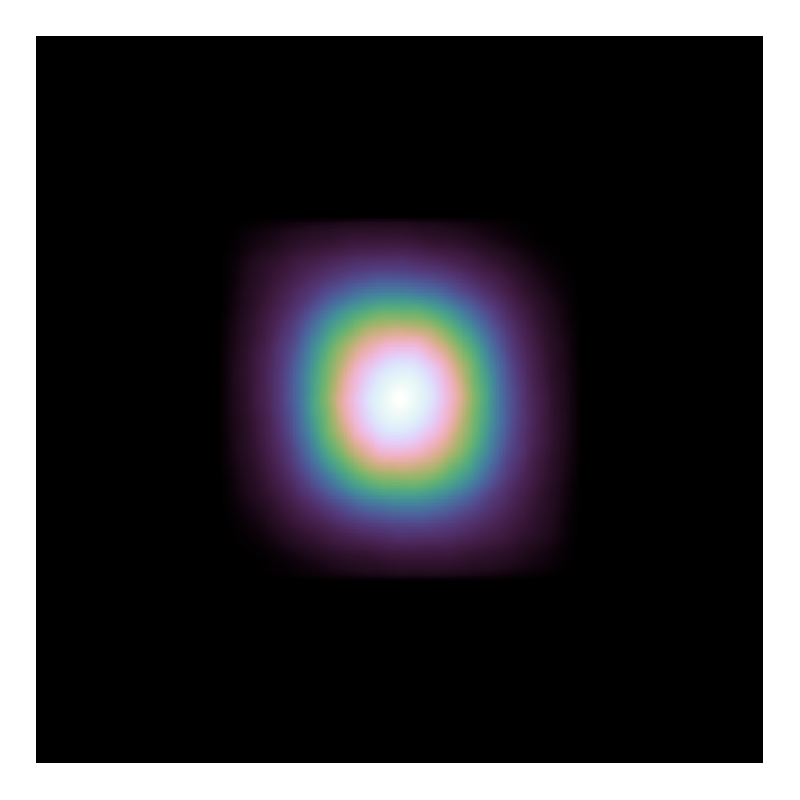
\includegraphics[width=\linewidth, clip, trim= 0.25in 0.25in 0.25in 0.25in]{./chapters/03.cd/simulated/psfSquaredCut.png}
		\caption{Approx. update}
	\end{subfigure}
	
	\caption{Approximation of gradient update.}
\end{figure} 

The basic coordinate descent method first correlates the residuals with the $PSF$. It pre-calculates the gradient for each pixel. Then, in each iteration, it directly updates the map of gradients with the product of $PSF \star PSF$ (the $PSF$ correlated with itself). In this approximation method, we start from the same pre-calculated map of gradients, but use an approximate update. The first coordinate descent iteration of this approximation method is identical to coordinate descent with the full $PSF$. With each coordinate descent iterations, the gradient map becomes more inaccurate. But with enough major cycles, this method converges to the same result as when the full $PSF$ is used.

The question is, how do we approximate the product of $PSF \star PSF$. As we have seen before, the product of $PSF \star PSF$ also approaches zero away from the center (an example was shown in Figure \ref{cd:efficient:update:figure} in Section \ref{cd:efficient:update}). A naive way to approximate the update step is to cut off the insignificant value and only use a rectangle of the center, which is a fraction of the total image size. For example: An image of size $1024^2$ also has a $PSF$ the size of $1024^2$. The product $PSF \star PSF$ actually has the size of $2048^2$ pixels due to the correlation. We can try to approximate the product by only using the center rectangle $\frac{1}{8}$ of the total size, ($256^2$ pixels). This approximation works, but leads to artifacts during deconvolution: The image will be reconstructed in visible "blocks" which are the size of the center fraction we use. 

We use the approximation shown in equation \eqref{gradient:method1:psf2}, where $cut()$ is the function that cuts away everything but the center rectangle of the $PSF$. This is a better approximation than cutting the product of $PSF \star PSF$ directly, and leads to faster convergence.

\begin{equation}\label{gradient:method1:psf2}
PSF \star PSF \approx cut(PSF) \star cut(PSF)
\end{equation}

The reason why \eqref{gradient:method1:psf2} is a better approximation lies in the reason why we update the gradients with the product of $PSF \star PSF$ in the first place: It is the combination of two separate operations, removing the $PSF$ from the residuals at the current position, and recalculating the correlation with the $PSF$. If we cut away parts of the product $PSF \star PSF$ directly, we implicitly update the residuals with a different $PSF$. But when we approximate the product by \eqref{gradient:method1:psf2}, we ensure that the implicit removal of the $PSF$ from the residuals is equal to $cut(PSF)$.

In our implementation, we use one more trick to improve the approximation: we scale the product of $cut(PSF) \star cut(PSF)$ to have the same maximum as the original product $PSF \star PSF$. The approximation has a lower maximum value than the original. Over several coordinate descent iterations, we run into the danger of over-estimating the pixel values. By scaling the product of $cut(PSF) \star cut(PSF)$ to the same maximum, we end up with a better approximation of the true gradient update.

\subsection{Method 2:Approximate deconvolution}
\begin{figure}[h]
	\centering
	\begin{subfigure}[b]{0.3\linewidth}
		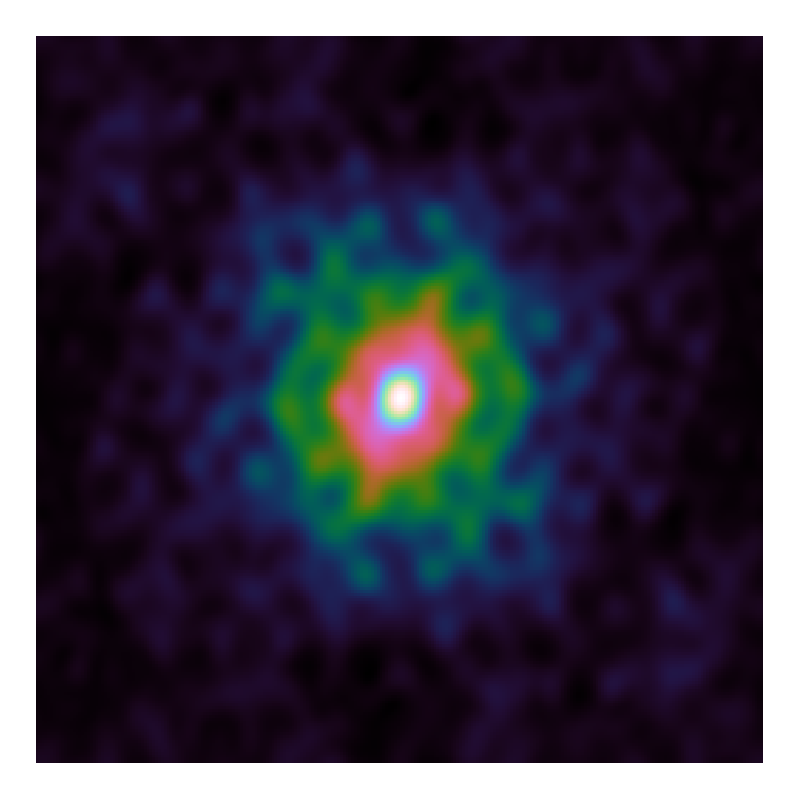
\includegraphics[width=\linewidth, clip, trim= 0.25in 0.25in 0.25in 0.25in]{./chapters/03.cd/simulated/psf.png}
		\caption{$PSF$ on log scale}
	\end{subfigure}
	\begin{subfigure}[b]{0.3\linewidth}
		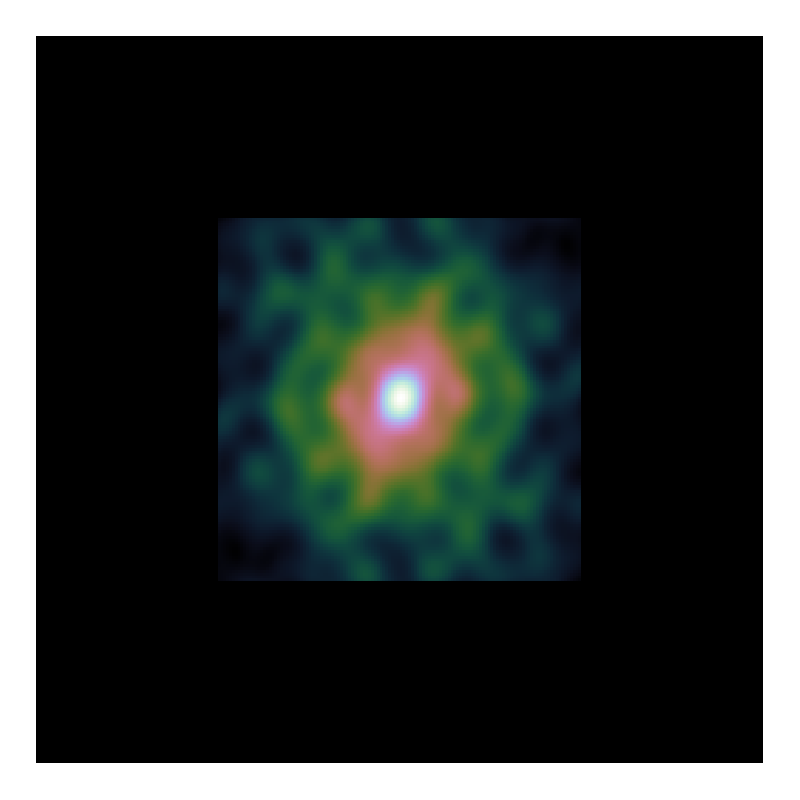
\includegraphics[width=\linewidth,clip, trim= 0.25in 0.25in 0.25in 0.25in]{./chapters/03.cd/simulated/psfCut.png}
		\caption{$\frac{1}{2}$ Fraction of the $PSF$}
	\end{subfigure}
	
	\caption{Approximate deconvolution with fraction $\frac{1}{2}$ of the $PSF$.}
\end{figure} 
The main problem with Method 1 is that the map of gradients becomes less accurate with more coordinate descent iterations. This method sovles this problem by using an approximate deconvolution instead, but it loses the guarantee to converge to the same result as the full $PSF$.

This method cuts off the insignificant part of the $PSF$, and only uses the center rectangle of it for the whole deconvolution problem. As such, the coordinate descent method solves an approximate deconvolution problem shown in \eqref{gradients:method2:objective}.

\begin{equation}\label{gradients:method2:objective}
\underset{x}{minimize} \: \frac{1}{2} \left \| I_{dirty} - x * cut(PSF) \right \|_2^2 + \lambda ElasticNet(x)
\end{equation}

In essence, it uses the same basic coordinate descent method, but ignore large parts of the $PSF$. It pre-calculates the gradient map by correlating the residual image with $cut(PSF)$, and update the gradient map with the product of $cut(PSF) \star cut(PSF)$. The main difference between approximate gradient update and approximate deconvolution is: In approximate gradient update starts with the same gradient map as the original. The approximate deconvolution does not. With this method, the gradient map does not become more inaccurate with more coordinate descent iterations.

The approximate deconvolution objective \eqref{gradients:method2:objective} is not guaranteed to "point" to the same solution as the original. It may in reality point to a very different solution. But thanks to the Major cycle, the image retrieved by optimizing \eqref{gradients:method2:objective} is always "close" to the original solution.

Nevertheless, this approximation method introduces an error in the final reconstructed image. The obvious error it introduces is it under-estimates the true pixel values. Pre-calculating the gradient map with $cut(PSF)$ under-estimates gradient magnitudes, and by extend the pixel values.

To combat the under-estimation of pixel values, we reduce the regularization parameter $\lambda$ for the approximate deconvolution problem. Since we cut off parts of the $PSF$, we also reduce the Lipschitz constant (sum of the squared $PSF$ values) used in the approximate deconvolution. We reduce the $\lambda$ parameter by the same factor that the Lipschitz constant gets reduced. This ensures that the approximate deconvolution and the original deconvolution arrive at the same pixel value for a point source. But it does not completely remove the issue for extended emissions.

\subsection{Major Cycle convergence and implicit path regularization}\label{gradients:pathreg}
In the two presented methods, we use a fraction of the $PSF$ to approximate the deconvolution problem. Both methods rely on the Major Cycle to periodically reset the gradient map. By using only a fraction of the $PSF$, the approximate deconvolution leaves parts of the $PSF$ in the gradient map. Figure \ref{gradient:convergence:sidelobe} shows the fraction of the $PSF$ that get included in the deconvolution, and "sidelobes" which get ignored.

%re-introduce residuals

\begin{figure}[h]
	\centering
	\begin{subfigure}[b]{0.3\linewidth}
		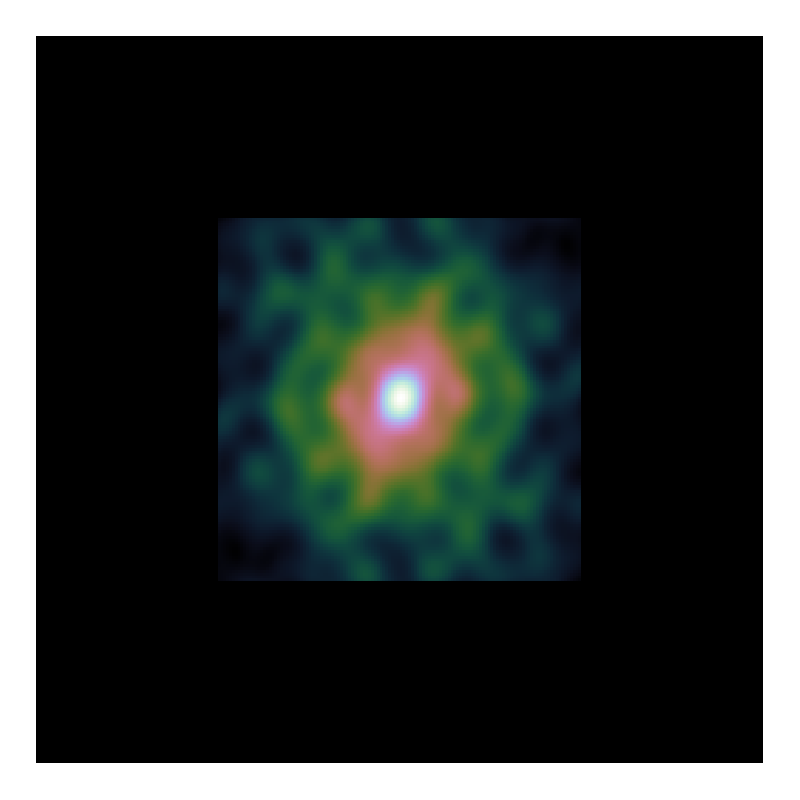
\includegraphics[width=\linewidth, clip, trim= 0.25in 0.25in 0.25in 0.25in]{./chapters/03.cd/simulated/psfCut.png}
		\caption{$\frac{1}{2}$ Fraction of the $PSF$}
	\end{subfigure}
	\begin{subfigure}[b]{0.3\linewidth}
		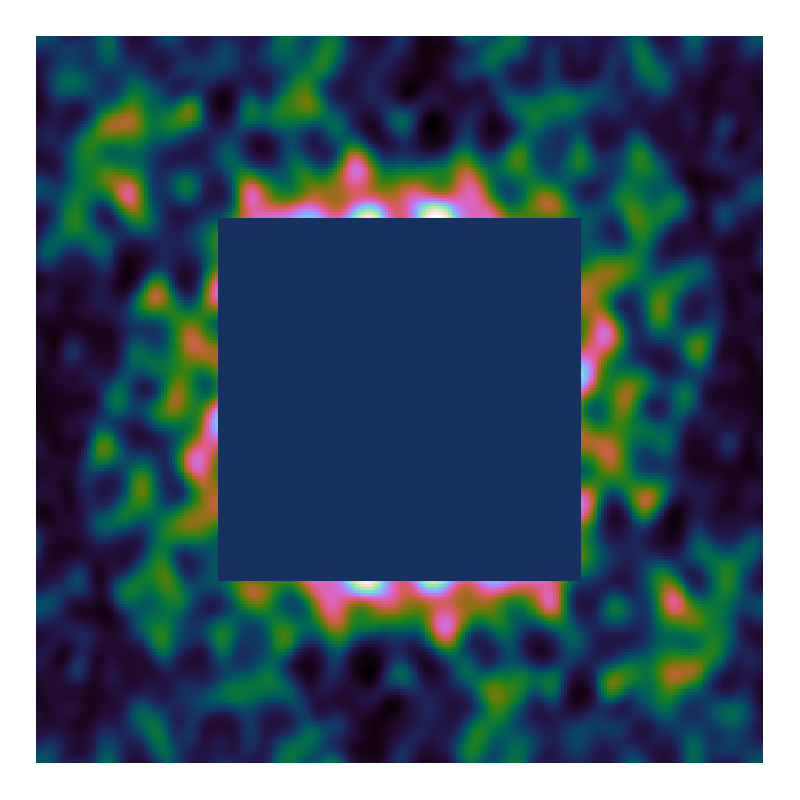
\includegraphics[width=\linewidth, clip, trim= 0.25in 0.25in 0.25in 0.25in]{./chapters/03.cd/simulated/psfReverseCut.png}
		\caption{$PSF$ Sidelobes}
		\label{gradient:convergence:reverseCut}
	\end{subfigure}
	
	\caption{Max sidelobe of the $PSF$ cutoff.}
	\label{gradient:convergence:sidelobe}
\end{figure}

After a number of serial coordinate descent iterations, we run into the danger of deconvolving the leftovers of the $PSF$ approximation. In that case, the serial coordinate descent algorithm adds spurious point sources to the image. After a major cycle, we can detect them as spurious and remove them again.
Degree to how bad this is depends on the maximum absolute value we cut off in the approximation, the maximum absolute value in Figure \ref{gradient:convergence:reverseCut}. With an aggressive approximation, we may end up oscillating from major cycle to major cycle: Adding spurious pixels and removing them again in the next, just to add the same spurious pixels in the one after.

But we can estimate at what point we are likely to add spurious pixels. This lets us estimate a minimum $\lambda$ parameter for the elastic net regularization. At this major cycle iteration, we cannot go below the minimum lambda. The next major cycle, the maximum residual is lower, and so is the minimum $\lambda$

This is known as a path regularization. We start with a stronger regularization and continually reduce $\lambda$ until we reached the desired value. We have intermediate results in each major cycle. Coordinate descent methods tend to be faster from a warm start, when we start from an intermediate result \cite{friedman2010regularization}. 

In this work we use the path regularization mainly for convergence of the major cycle. 

How we estimate the minimum $\lambda$ parameter. Imagine the interferometer only observed a point source in the center of the image. In that case, 
after the first serial coordinate descent iteration, our residuals image looks exactly like the Figure \ref{gradient:convergence:reverseCut}. The serial coordinate descent algorithm should not take another step, or it adds spurious pixels. In other words, the regularization has to suppress all the values in Figure \ref{gradient:convergence:reverseCut}

Remember the elastic net regularization: It is a mixture of the L1 and L2 norm. The L1 norm shrinks the pixel values, while the L2 norm divides them. We need the L1 norm to shrink away the values in Figure \ref{gradient:convergence:reverseCut}.

\begin{equation}
\begin{split}
gradients &= residuals \star PSF \\
maxSidelobe &= Max(gradients) * Max(Abs(Sidelobe(PSF)))) \\
\lambda_{cycle} &= \frac{maxSidelobe}{\alpha}
\end{split}
\end{equation}

This estimate is a minimum. Meaning it is possible that we still add spurious pixels. For example when the sidelobes of two point sources overlap.

The estimate however only considers point sources. For extended emissions, the estimate is too low. Extended emissions are a group of non-zero pixels. Beause they are next to each other, their sidelobes overlap and get amplified. 

An estimate considering extended emissions.

\begin{equation}
\begin{split}
psfSidelobe &= Max(PSF - cut(PSF)) \\
gradients &= residuals \star PSF \\
correction &= Max(1, \frac{Max(gradients)}{Max(residuals) * lipschitz}) \\
maxSidelobe &= Max(gradients) * Max(psfSidelobe) * correction \\
\lambda_{cycle} &= \frac{maxSidelobe}{\alpha}
\end{split}
\end{equation}

Only considers the "maximum" extended emission. Extended emissions tend to contain the largest pixel value in the residual image. Because of the convolution.
The correction factor gets reduced the closer the maximum pixel in the residuals. Over several major cycles, the correction factor and the $lambda_{cycle}$ become smaller. 
Helps convergence.


But this is not true for extended emissions.

he serial deconvolution algorithm calculates the gradient map (by correlating the $PSF$ with the residuals).


Residuals will be left. 



